\section{Pc}
\subsection{GUI}
\begin{figure}[H]
\centering
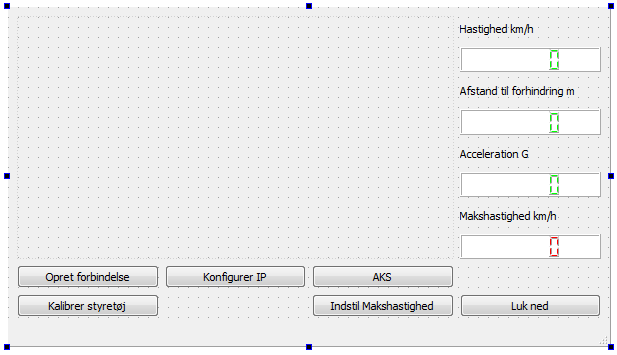
\includegraphics[width=\textwidth* 3/4,height=\textwidth* 9/20 ]{../fig/billeder/gui_design.png}
\caption{GUI i implementerings processen}
\label{fig:GUI_design}
\end{figure}
Udviklingsmiljøet som hele GUI'en er skrevet i er Qt version 5.5 \cite{lib:qt}. En af fordelene ved QT er at man kan lave den grafiske del af GUI'en hurtigt og uden at skulle vide noget om hvordan koden bagved fungerer. Princippet er drag and drop og fungerer ved at man trækker de forskellige knapper og bokse ind i vinduet. Qt opretter selv en klasse kaldet MainWindow. I Main.cpp oprettes en instans af MainWindow som gør at hele programmet køres i MainWindow's constructor. Når programmet kører og der trykkes på en knap gives der et signal. Signalet forbindes til en slot i constructoren ved hjælp af funktionen \texttt{connect}.
\begin{lstlisting}[caption={Forbindelse af signals og slots},label=gui_connect, language=c++]
connect(ui->OpretForbindelse, SIGNAL(clicked()), this, SLOT(Au2connect()));
connect(ui->KonfigurerIP, SIGNAL(clicked()), this, SLOT(konfigurerIP()));
connect(ui->AKS, SIGNAL(clicked()), this, SLOT(AKSstatus()));
connect(ui->IndstilMaksHastighed, SIGNAL(clicked()), this, SLOT(maksHastighed()));
connect(ui->KalibrerStyretoj, SIGNAL(clicked()), this, SLOT(kalibrerStyretoj()));
connect(ui->LukNed, SIGNAL(clicked()), this, SLOT(shutDown()));
connect(this, SIGNAL(sig_getData()), this, SLOT(readSocket()));
\end{lstlisting}
I listing \ref{gui_connect} ses fx. at når der klikkes på OpretForbindelse kaldes funktionen Au2connect som er funktionen der opretter forbindelsen til bilen. 



\subsection{VLC}
Udviklingsmiljøet som hele GUI'en er skrevet i er Qt version 5.5. For at inkludere VLC, skal Qt være installeret \cite{lib:qt}. For at kunne modtage video stream i GUI'en skal vi bruge en forbygget version af VLC til windows32 indeholdende .dll filer osv, samt bilioteker til Qt. Dette gøres ved at udpakke Filen \textbf{vlc-2.0.7-win32.7z} som hentes fra en ftp server \cite{lib:vlc-ftp}. til destinationen \textbf{c:/Qt/}. Pakken indeholder rumtime-filerne som senere skal kopieres over i debugfolderen. Include filerne til Qt downloades \textbf{“Official VLC-Qt Windows SDK and Source Packages”} \cite{lib:vlc-qt} og udpakkes i \textbf{c:/Qt/}. I denne pakke ligger der et demoprojekt som der er hentet inspiration fra til projektet. Laves der et nyt projekt skal der inkluderes de rigtige filer til Qt. Dette gøres ved at åbne .pro filen i Qt og tilføje:

\begin{lstlisting}
# Edit below for custom library location
LIBS     += -LC:\Qt\libvlc-qt\lib -lvlc-qt -lvlc-qt-widgets
INCLUDEPATH += C:\Qt\libvlc-qt
\end{lstlisting}
Når projektet er bygget kopieres filerne \textbf{libvlc-qt-widgets.dll} og \textbf{libvlc-qt.dll} fra \textbf{C:/Qt/libvlc-qt/bin} til build folderen. Efterfølgende kopieres filerne \textbf{axvlc.dll, libvlc.dll, libvlccore.dll} og \textbf{npvlc.dll} fra \textbf{C:/Qt/vlc-2.0.7} samt folderen \textbf{plugins} også til buildfolderen. Programmet skulle nu genre kunne køre. Hvis ikke kan der findes mere hjælp her \cite{lib:vlc-using-qt}. Desværre er der nogle fejl i linket, som der gerne skulle være rettet i denne beskrivelse. 